\documentclass[12pt]{article}
\usepackage{graphicx}
\usepackage{subcaption}
\usepackage{mwe}
%\usepackage{lingmacros}
%\usepackage{tree-dvips}
%\usepackage{blindtext}
%\usepackage[utf8]{inputenc}

\begin{document}

\title{HW0: Pin It!}
\author{Gudjon Einar Magnusson}

\maketitle


\section{Denoise}

Filtering out the noise is not strictly speaking needed to get the job done but it produces a slightly cleaner result. To filter the noise I used the \textit{medfilt2} function, mainly because its very simple. \textit{medfilt2} operates on a 2D matrix a therefore I apply it to each channel of the RGB image separately and then recombine the filtered channels for the final result. Figure \ref{fig_denoise} shows the image before and after the noise filter.

\begin{figure}
    \begin{subfigure}{.5\textwidth}
        \centering
        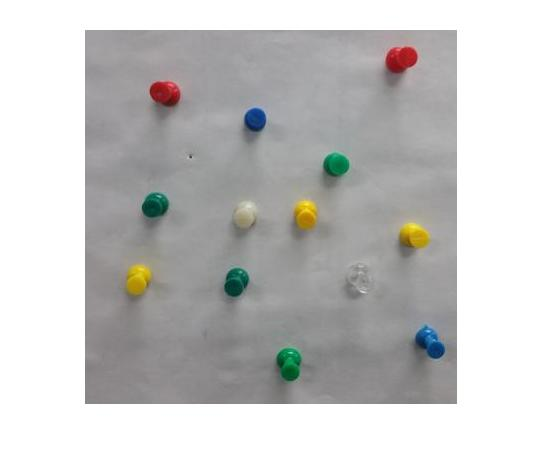
\includegraphics[width=\linewidth]{pins_original}
        \caption{Original pins image}
    \end{subfigure}\hfill
    \begin{subfigure}{.5\textwidth}
        \centering
        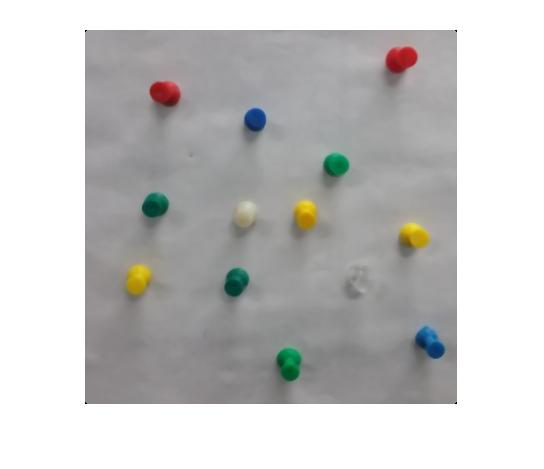
\includegraphics[width=\linewidth]{pins_filt}
        \caption{Pins image after noise filter}
    \end{subfigure}
    \caption{This shows the subtle effect of the noise filter}
    \label{fig_denoise}
\end{figure}


\section{Find the pins}

\subsection{Color Normalization}
To start with I want to find all pins in the image, of any color. To do this I came up with a very simple normalization function. For each pixel of the image I divided the minimum value of any channel with mean value of all the channels. This is a very effective way to separate colored pixels from white pixels. White and gray pixels have a high value close the the average in each color channels but bright colors have more variable values in each channel. This produces a gray-scale image where bright colors appear very dark and white and gray appears very bright. Figure \ref{fig_norm} shows the image before and after normalization.
Unfortunately, as you can see, this normalization function does not do a good job of finding the white and transparent pins.

\begin{figure}
    \begin{subfigure}{.5\textwidth}
        \centering
        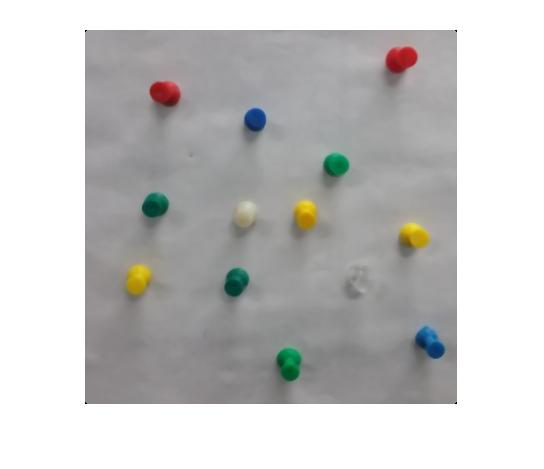
\includegraphics[width=\linewidth]{pins_filt}
        \caption{Color image}
    \end{subfigure}\hfill
    \begin{subfigure}{.5\textwidth}
        \centering
        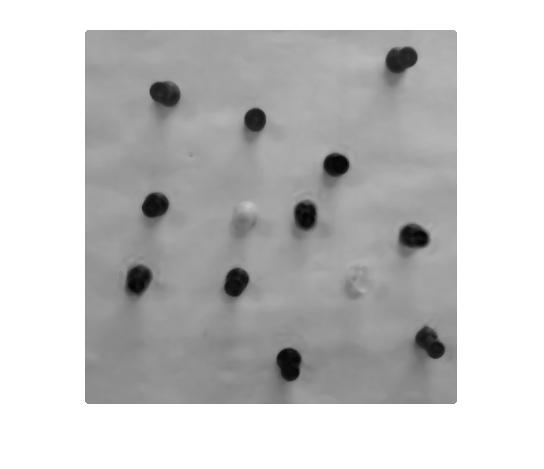
\includegraphics[width=\linewidth]{pins_norm}
        \caption{Normalized image}
    \end{subfigure}
    \caption{This shows the effect of the normalization function}
    \label{fig_norm}
\end{figure}

\subsection{Separate the pins}

To separate pins from the background and localize them, I produce a binary image where 1 in pin and 0 is background. I do this by using the \textit{im2bw} function. \textit{im2bw} take a 2D matrix and threshold value. Any pixel with a value greater than the threshold becomes a 1 and any value below becomes a 0. With my normalization function a threshold of ${0.4}$ works well. With a slightly higher threshold I can just start to make out the white and clear pins, but I don't think thats a reliable result. Since the normalization function shows the pins as dark and the background as bight but I want the pins to be classified with a value of 1 I invert the resulting binary image using the logical NOT operator. Figure \ref{fig_bw} shows the image before and after applying the \textit{im2bw} function.

\begin{figure}
    \begin{subfigure}{.5\textwidth}
        \centering
        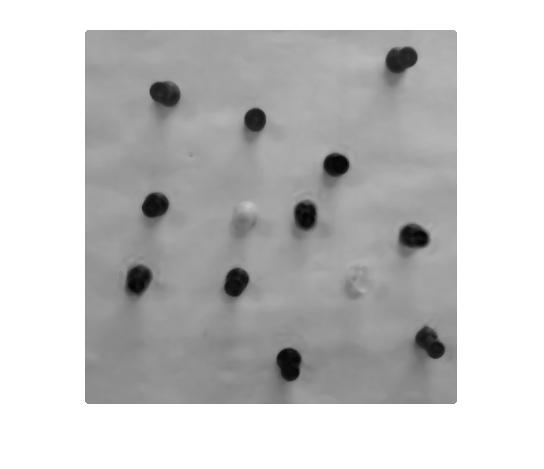
\includegraphics[width=\linewidth]{pins_norm}
        \caption{Normalized image}
    \end{subfigure}\hfill
    \begin{subfigure}{.5\textwidth}
        \centering
        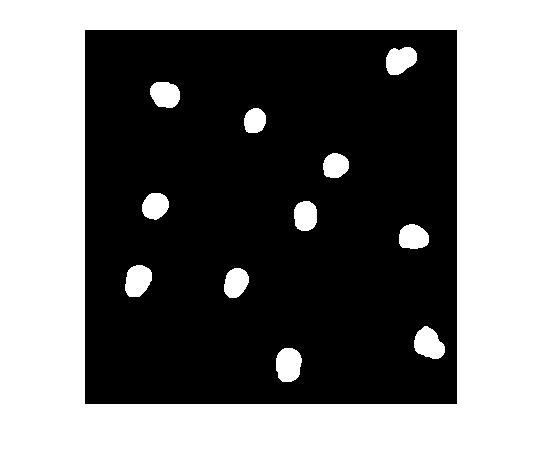
\includegraphics[width=\linewidth]{pins_bw}
        \caption{Binary image}
    \end{subfigure}
    \caption{The effect of applying a ${0.4}$ threshold to the normalized image.}
    \label{fig_bw}
\end{figure}


\subsection{Localize the pins}

To count an localize the pins in binary image I use the \textit{regionprops} function. \textit{regionprops} returns information about connected regions in a binary image, such a bounding box. With the bounding box I can draw a box around the pins and I'll do that after I figure out their color.


\section{Classify the pins}

To classify the color of the pins I look at each pin separately. I produce a small sub-image using the bounding box returned by the \textit{regionprops} function and calculate its mean color value. This gives me a single RGB vector for each pin. Next I calculate the euclidean distance between that vector and each of my 4 reference colors, red, green, blue and yellow. Which ever color has the smallest distance is the color of the pin. Now I can draw the bounding box using the \textit{rectangle} function.


\begin{figure}
    \centering
    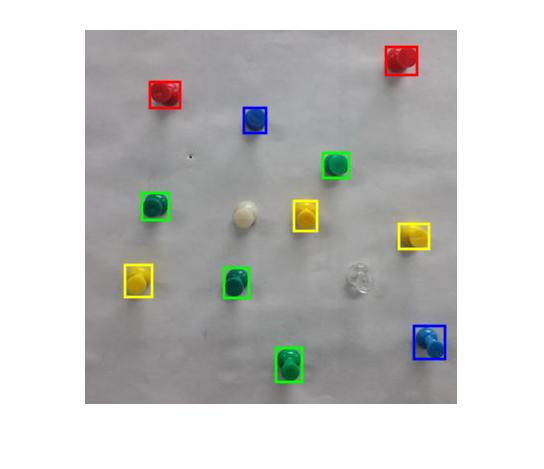
\includegraphics[width=3.0in]{pins_box2}
    \caption{Pins labeled with their classified color}
    \label{fig_pins_box2}
\end{figure}


\end{document}